% -*- LaTeX -*-
% -*- coding: utf-8 -*-
%
% ~~~~~~~~~~~~~~~~~~~~~~~~~~~~~~~~~~~~~~~~~~~~~~~~~~~~~~~~~~~~~~~~~~~~~~~~~~~~~~
%
%                             michael a.g. aïvázis
%                      california institute of technology
%                      (c) 1998-2010  all rights reserved
%
% ~~~~~~~~~~~~~~~~~~~~~~~~~~~~~~~~~~~~~~~~~~~~~~~~~~~~~~~~~~~~~~~~~~~~~~~~~~~~~~
%

\lecture{Programming with MPI}{20100125}

% --------------------------------------
% template
\begin{frame}[fragile]
%
  \frametitle{Distributed memory parallelism}
%
  \begin{itemize}
%
  \item recall the generic layout of a distributed memory machine
%
    \begin{figure}
      \centering
      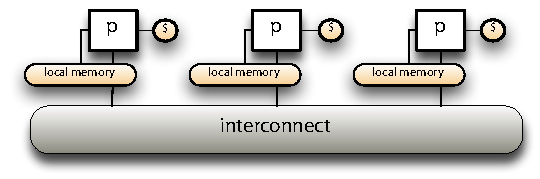
\includegraphics[scale=1.0]{figures/distributed-memory.pdf}
    \end{figure}
    \vspace{-1.0em}
%
    \begin{itemize}
      \item each processor has its own private memory space
      \item processors communicate via the interconnect substrate
    \end{itemize}
%
  \item the programming model
    \begin{itemize}
    \item program consists of a collection of $p$ named processes
      \item each process has its own instruction stream and address space
    \item logically shared data must be partitioned among the processors
    \item communication and synchronization must be orchestrated explicitly 
    \item processes communicate via explicit data exchanges
    \end{itemize}
%
  \end{itemize}
%
\end{frame}

% --------------------------------------
% template
\begin{frame}[fragile]
%
  \frametitle{\mpi\ -- the survivor}
%
  \begin{itemize}
%
  \item the {\em de facto} standard for writing parallel programs using message passing
    \begin{itemize}
    \item a library of routines callable from almost any programming language
    \item that enables communication among multiple processes
    \item standardized and portable API with good implementations available for almost any kind
      of parallel computer
    \end{itemize}
%
  \item \mpi\ is large and complex
    \begin{itemize}
    \item more than 125 functions, lot's of options and communication protocols
    \item but for most practical purposes, a small subset will suffice
    \item short introduction today, more when we consider specific physics
    \end{itemize}
%
  \item two major versions available -- check your installation for compliance
    \begin{itemize}
    \item \mpi\ 1: parallel machine management, process groups, collective operations,
      point-to-point operations, virtual topologies, profiling
    \item \mpi\ 2: dynamic process management, one-sided operations, parallel I/O, (simplistic)
      bindings for \cpp
    \end{itemize}
%
  \end{itemize}
%
\end{frame}

% --------------------------------------
% parallel machine management
\begin{frame}[fragile]
%
  \frametitle{Getting started}
%
  \begin{itemize}
%
  \item building:
    \begin{itemize}
    \item supplied wrappers
    \item on your own
    \end{itemize}
%
  \item staging:
    \begin{itemize}
    \item native: mpirun
    \item queue management:
    \end{itemize}
%
  \item launching:
    \begin{itemize}
    \item initialize: \function{MPI\_Init}, \identifier{MPI\_COMM\_WORLD}
    \item query the runtime environment
    \item finalize: \function{MPI\_Finalize}
    \end{itemize}
%
  \end{itemize}
%
\end{frame}

% --------------------------------------
% communicators
\begin{frame}[fragile]
%
  \frametitle{Communicators}
%
  \begin{itemize}
%
  \item 
%
  \end{itemize}
%
\end{frame}

% --------------------------------------
% hello world
\begin{frame}[fragile]
%
  \frametitle{Hello world}
%
  \label{slide:hello-world-mpi}
%
  \begin{C}
#include <mpi.h>
#include <stdio.h>

int main(int argc, char* argv[]) {
    int status;
    int rank, size;

    /* initialize MPI */
    status = MPI_Init(&argc, &argv);
    if (status != MPI_SUCCESS) {
        printf("error in MPI_Init; aborting...\n");
        return status;
    }

    /* all good */
    MPI_Comm_rank(MPI_COMM_WORLD, &rank);
    MPI_Comm_size(MPI_COMM_WORLD, &size);
    printf("hello from %03d/%03d!\n", rank, size);

    /* shut down MPI */
    MPI_Finalize();

    return 0;
}
  \end{C}
%
\end{frame}

% --------------------------------------
% example reduction with mpi
\begin{frame}[fragile]
%
  \frametitle{Example reduction using \mpi}
%
  \label{slide:hello-world-mpi}
%
  \begin{C}[basicstyle=\tt\bfseries\tiny]
#include <mpi.h>
#include <stdio.h>

int main(int argc, char* argv[]) {
    int status;
    int rank;
    int square, sum;

    /* initialize MPI */
    status = MPI_Init(&argc, &argv);
    if (status != MPI_SUCCESS) {
        printf("error in MPI_Init; aborting...\n");
        return status;
    }

    /* get the process rank */
    MPI_Comm_rank(MPI_COMM_WORLD, &rank);
    /* form the square */
    square = rank*rank;
    /* each process contributes the square of its rank */
    MPI_Allreduce(&square, &sum, 1, MPI_INT,  MPI_SUM, MPI_COMM_WORLD);
    /* print out the result */
    printf("%03d: sum = %d\n", rank, sum);

    /* shut down MPI */
    MPI_Finalize();

    return 0;
}
  \end{C}
%
\end{frame}

% end of file 
